%  CONFIGURE NEW SINGLE-PAGE FORMAT 

\onecolumn % go back to one column
\fancyhead{} % make sure we get no headers
\renewcommand{\floatpagefraction}{0.1}
\lfoot[\bSupInf]{\dAuthor}
\rfoot[\dAuthor]{\cSupInf}
\newpage

\captionsetup*{format=largeformat} % make figure legend slightly larger than in the paper
\setcounter{figure}{0} % reset figure counter for Supp. Figures
\setcounter{equation}{0} % reset equation counter for Supp. Equations
%\setcounter{page}{1} % reset page count
\makeatletter 
\renewcommand{\thefigure}{S\@arabic\c@figure} % make Figure legend start with Figure S
\makeatother
\def\theequation{S\arabic{equation}}

%  MAIN TEXT 

\newpage
\section*{Supplementary Figures}

\begin{figure*}[!ht]
\centering
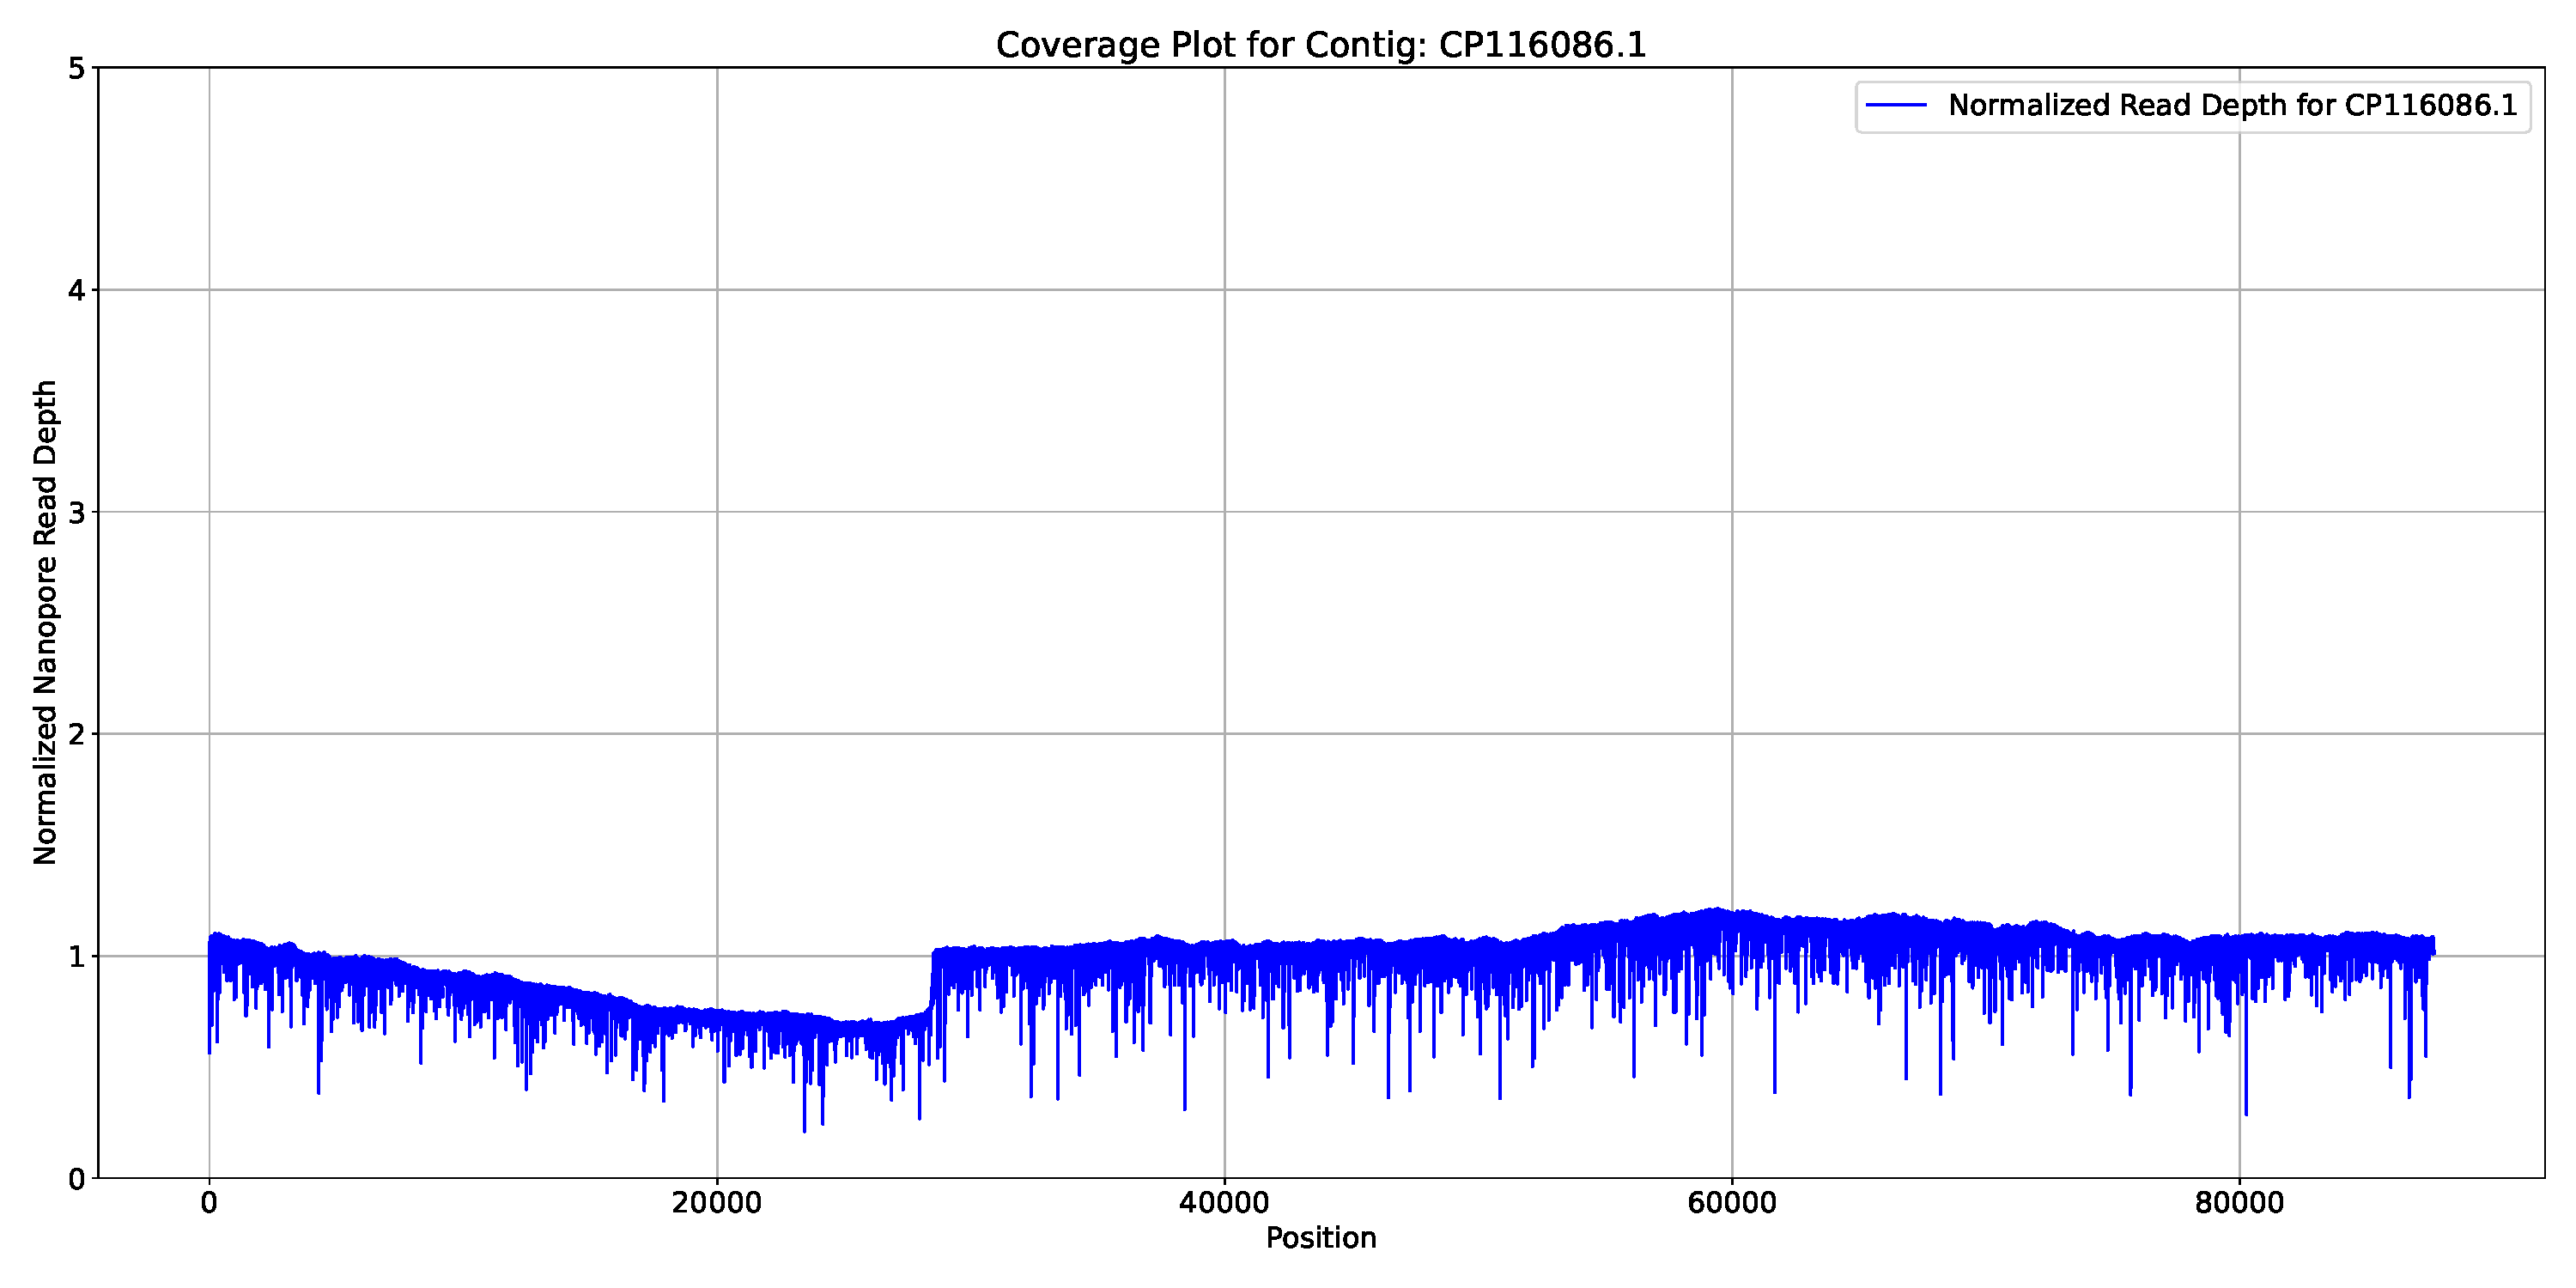
\includegraphics[width=0.75\linewidth]{Figures/figure_S1.pdf}
\caption{We identified a region of elevated coverage in contig CP116086.1 in sample GCA\_027944635.1\_ASM2794463v1\_genomic. We extracted the reads mapping to this region using \texttt{samtools view GCA\_027944635.1\_ASM2794463v1\_genomic.bam CP116086.1 | cut -f1 | sort | uniq} and subsetted the nanopore FASTQ to just these reads using pyfastaq \texttt{filter}. We reassembled the reads using Canu \texttt{v2.3} with \texttt{genomeSize=100k} and short-read polished the resulting contig with polypolish \texttt{v0.6.0}. We then directly replaced CP116086.1 with this contig.}
\label{suppfig:1}
\end{figure*}

\begin{figure*}[!ht]
\centering
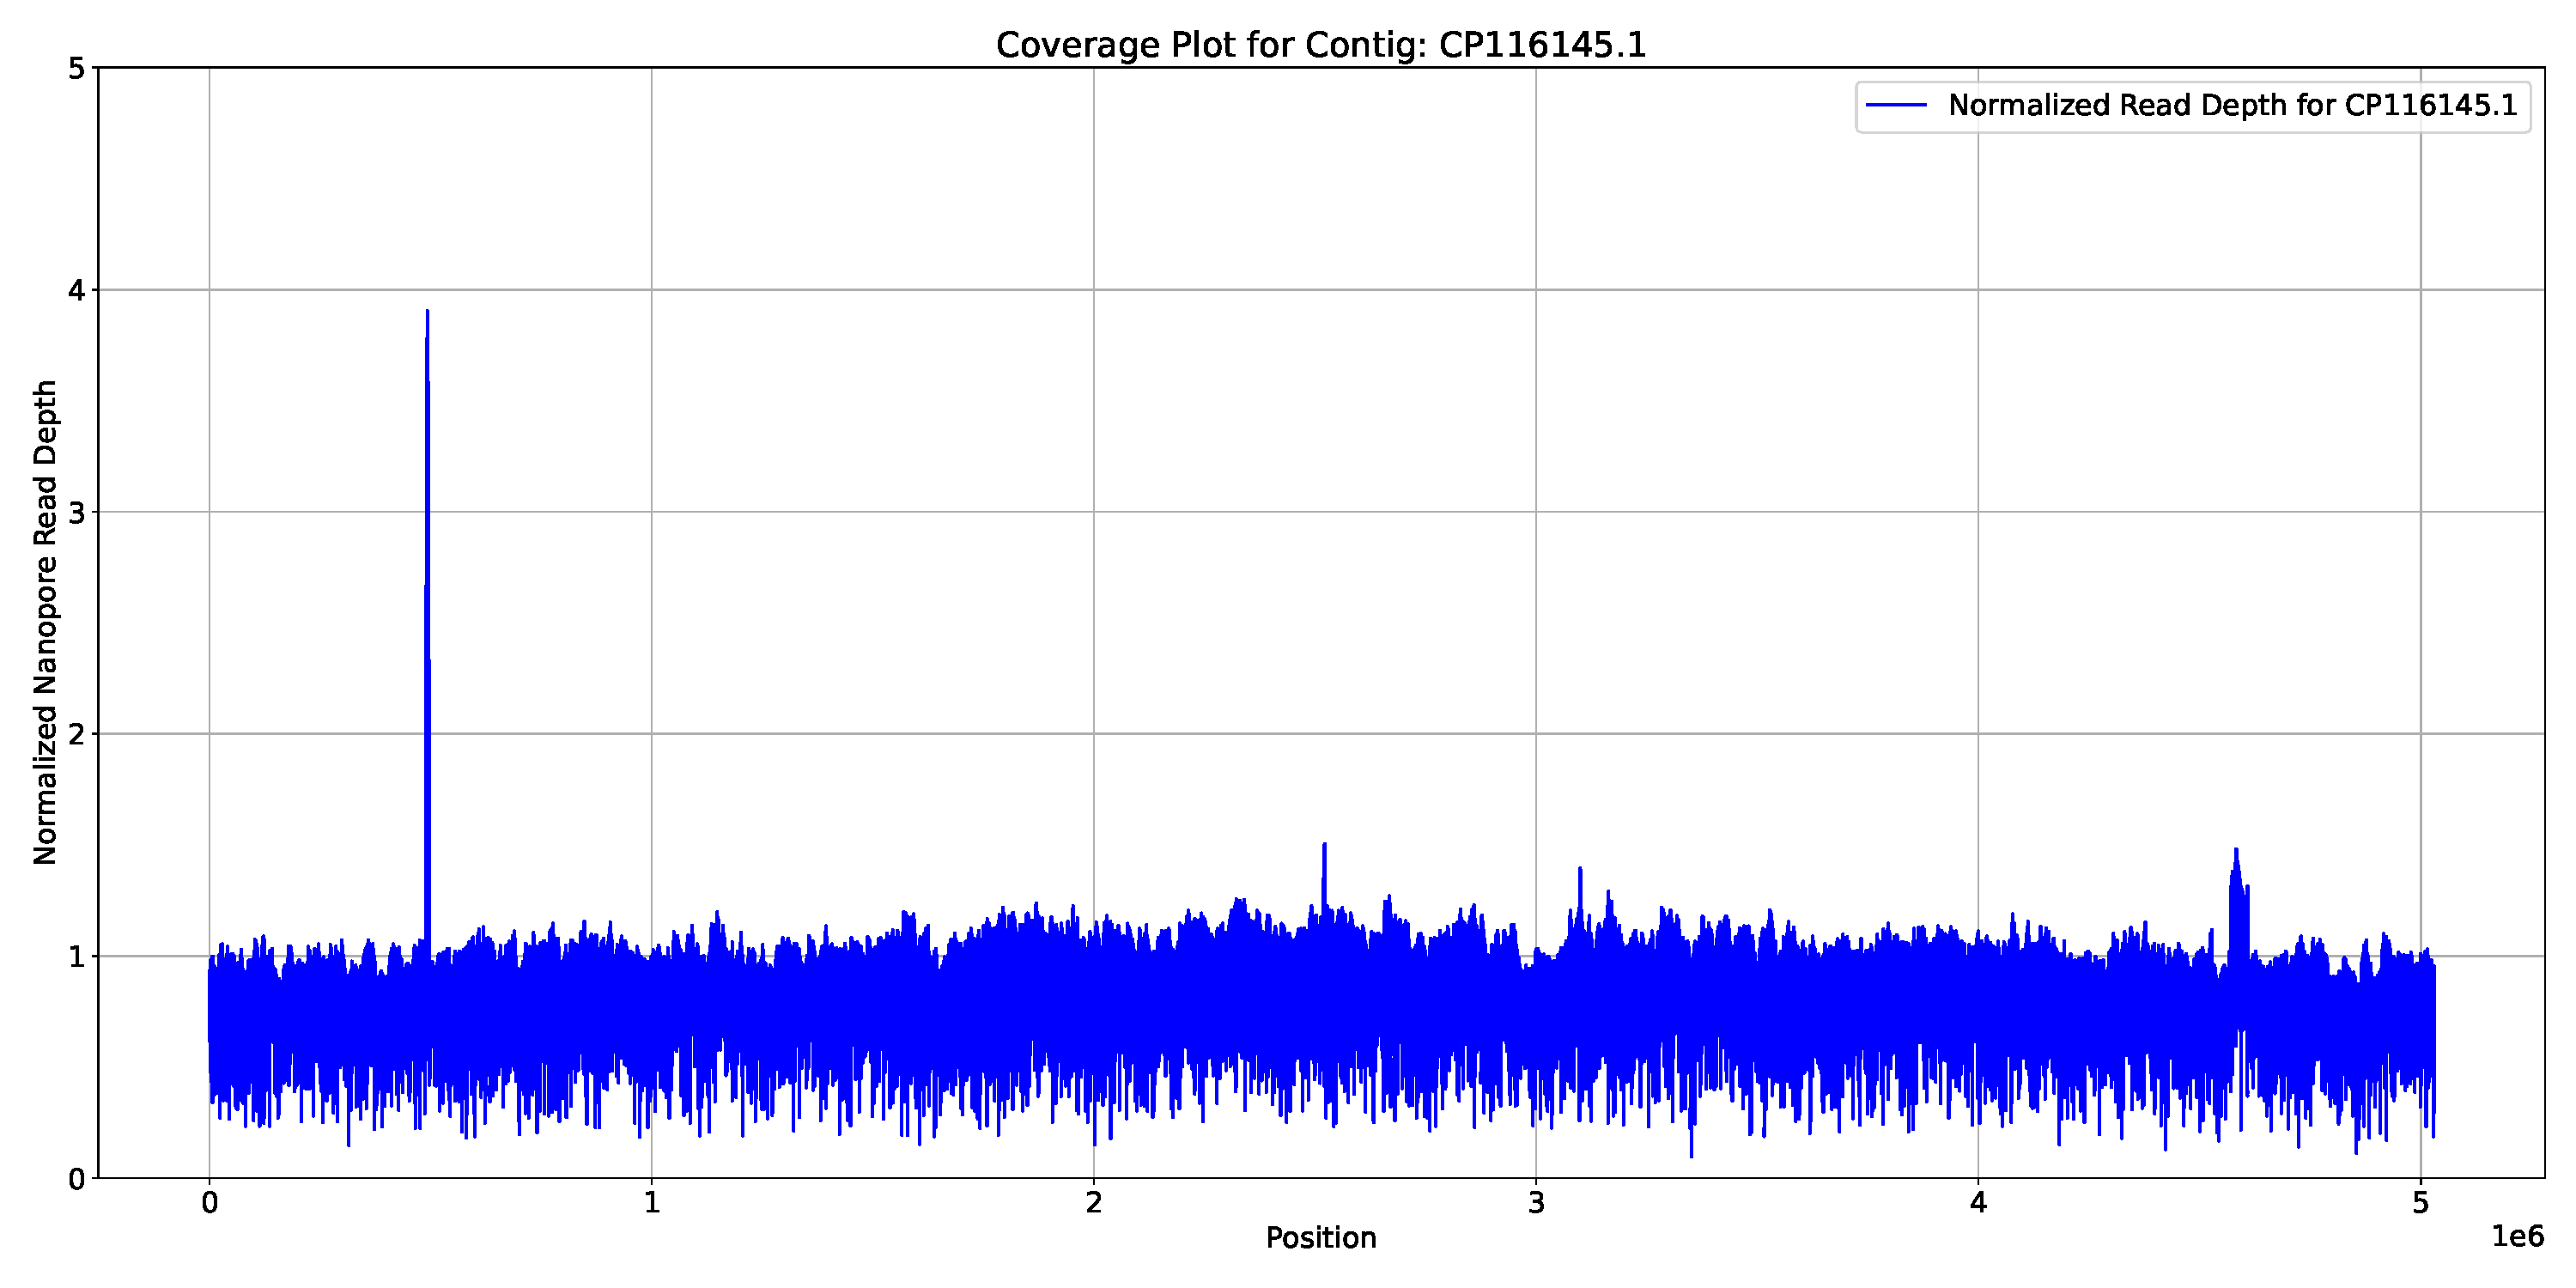
\includegraphics[width=0.75\linewidth]{Figures/figure_S3.pdf}
\caption{We identified a region of elevated coverage in contig CP116145.1 in sample GCA\_027944835.1\_ASM2794483v1\_genomic. We extracted the soft-clipped reads mapping to this region using \texttt{samtools view -f 2048 -f 2064 GCA\_027944835.1\_ASM2794483v1\_genomic.bam CP116145.1:300000-700000 | cut -f1 | sort | uniq} and subsetted the nanopore FASTQ to just these reads using pyfastaq \texttt{filter}. We reassembled the reads using flye \texttt{v2.9.3} \texttt{--iterations 3}. We visualised the alignment between the assembly and the reference using TNA \texttt{v0.3.0}, and found it fully covered plasmid contig CP116148.1 with 99.9\% identity so was not evident of a collapsed duplication.}
\label{suppfig:3}
\end{figure*}

\begin{figure*}[!ht]
\centering
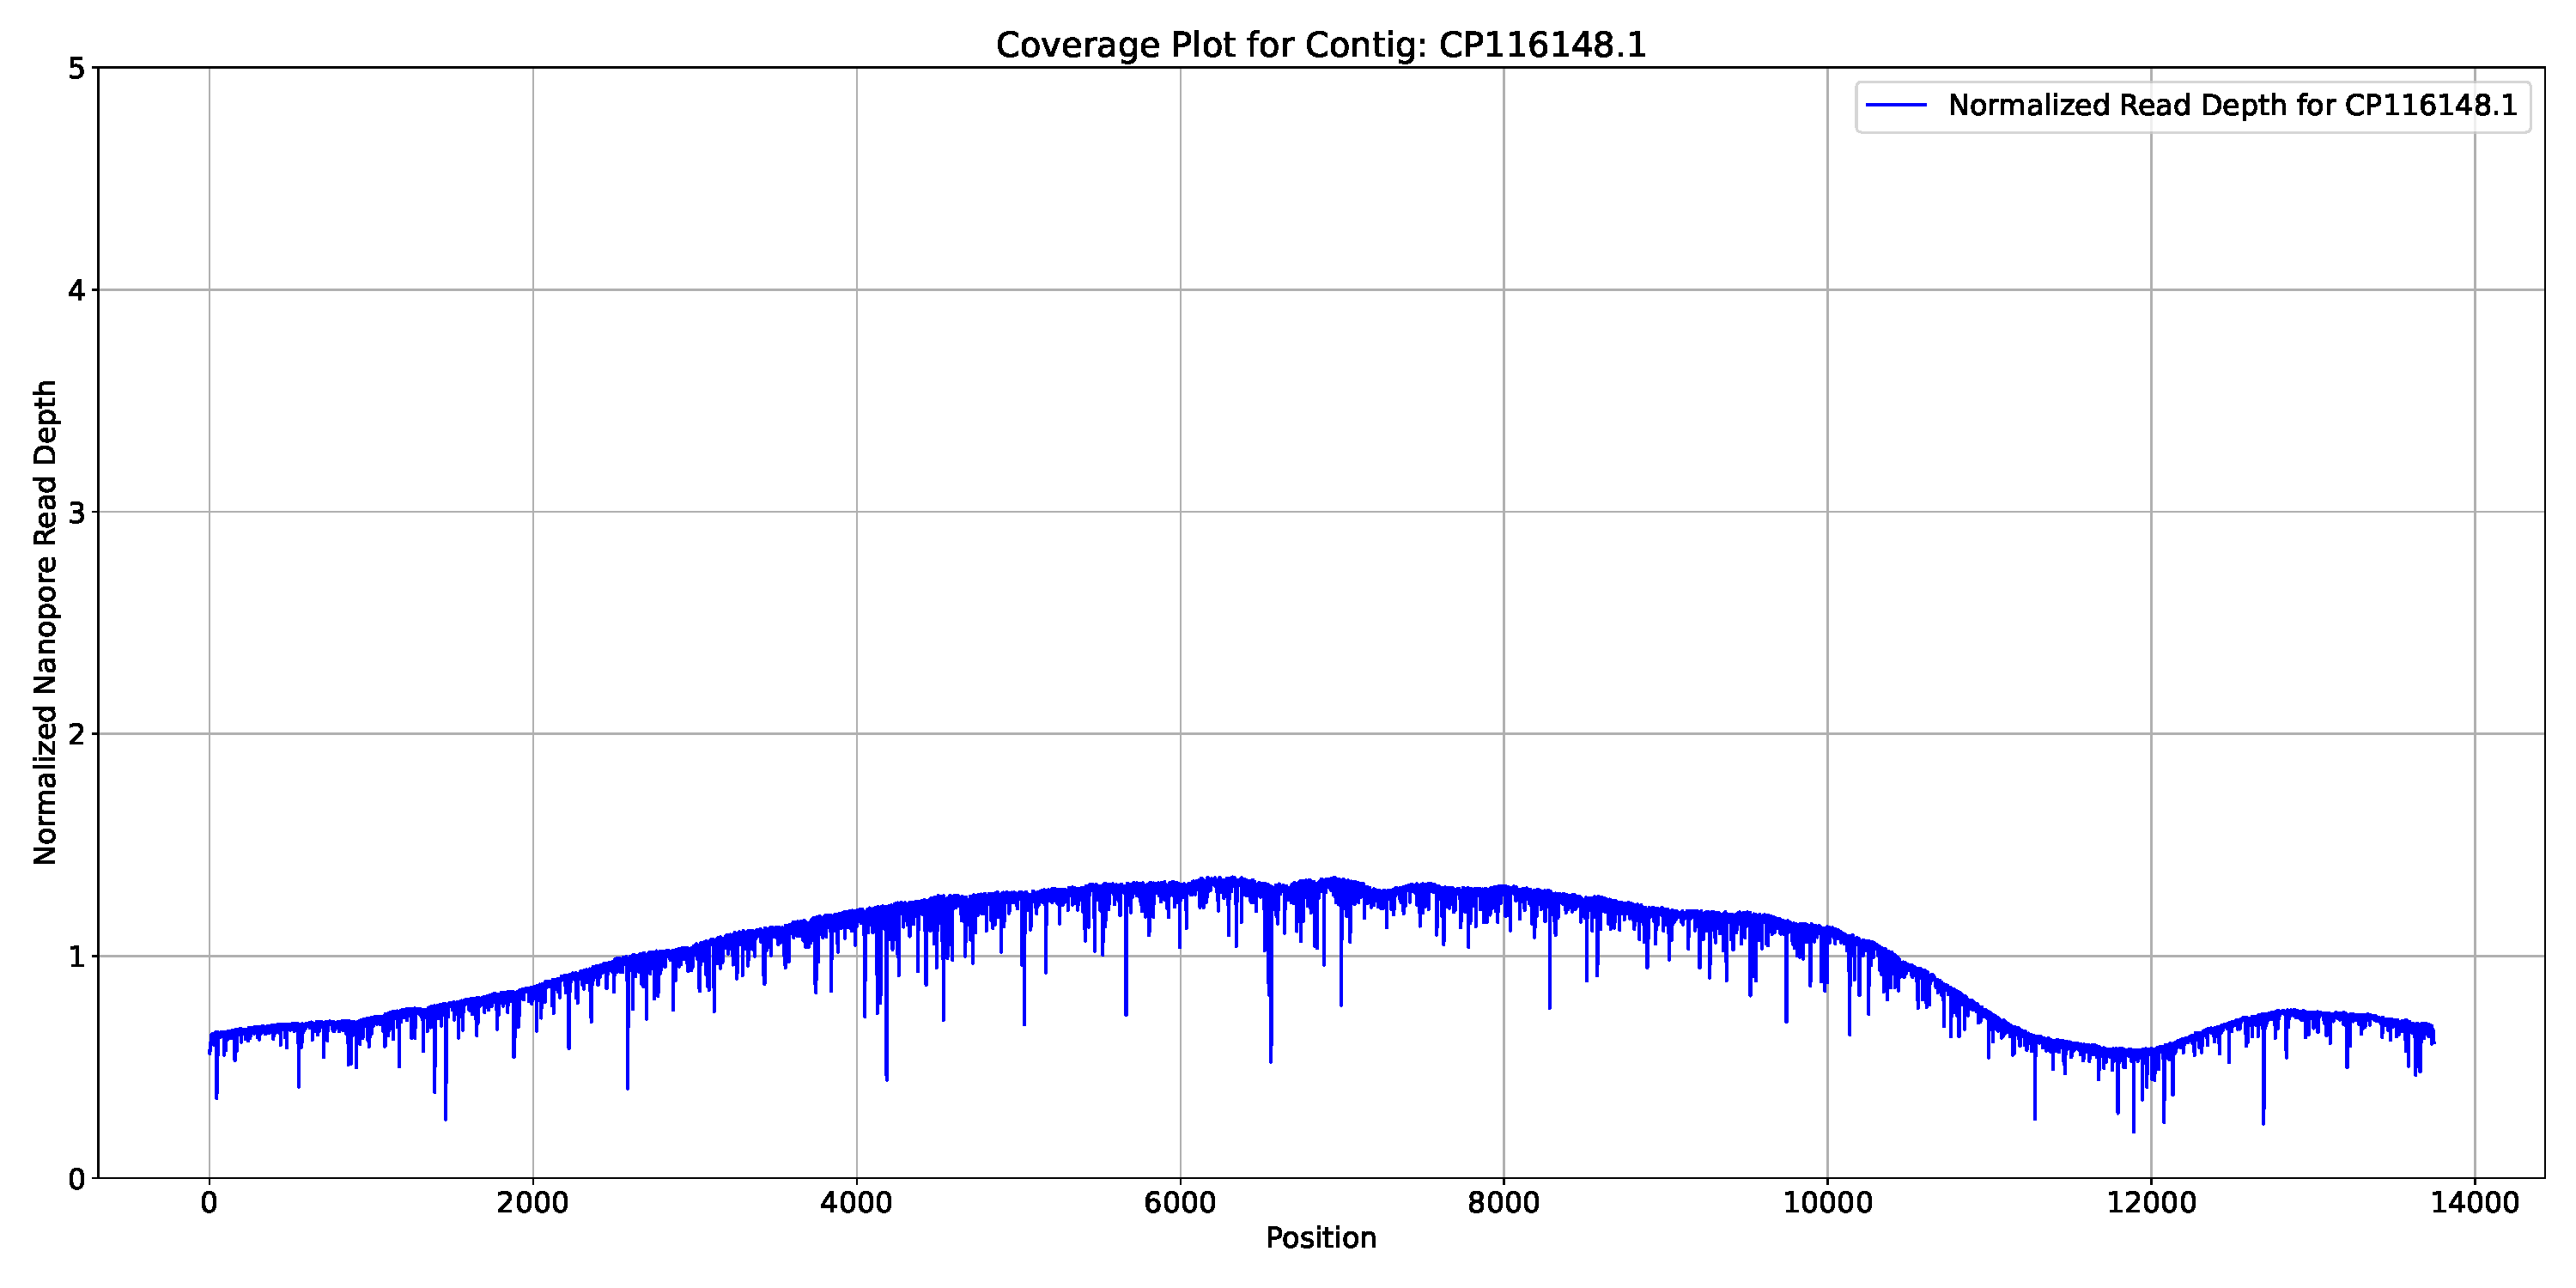
\includegraphics[width=0.75\linewidth]{Figures/figure_S4.pdf}
\caption{We identified a region of elevated coverage in contig CP116148.1 in sample GCA\_027944835.1\_ASM2794483v1\_genomic. We subsetted the reads mapping to the contig using \texttt{samtools view GCA\_027944835.1\_ASM2794483v1\_genomic.bam CP116148.1 | cut -f1 | sort | uniq} and pyfastaq \texttt{filter}. We reassembled the reads using Canu \texttt{v2.3} with \texttt{genomeSize=20k} and short-read polished the resulting contig with polypolish \texttt{v0.6.0}. We then directly replaced CP116148.1 with this contig.}
\label{suppfig:4}
\end{figure*}

\begin{figure*}[!ht]
\centering
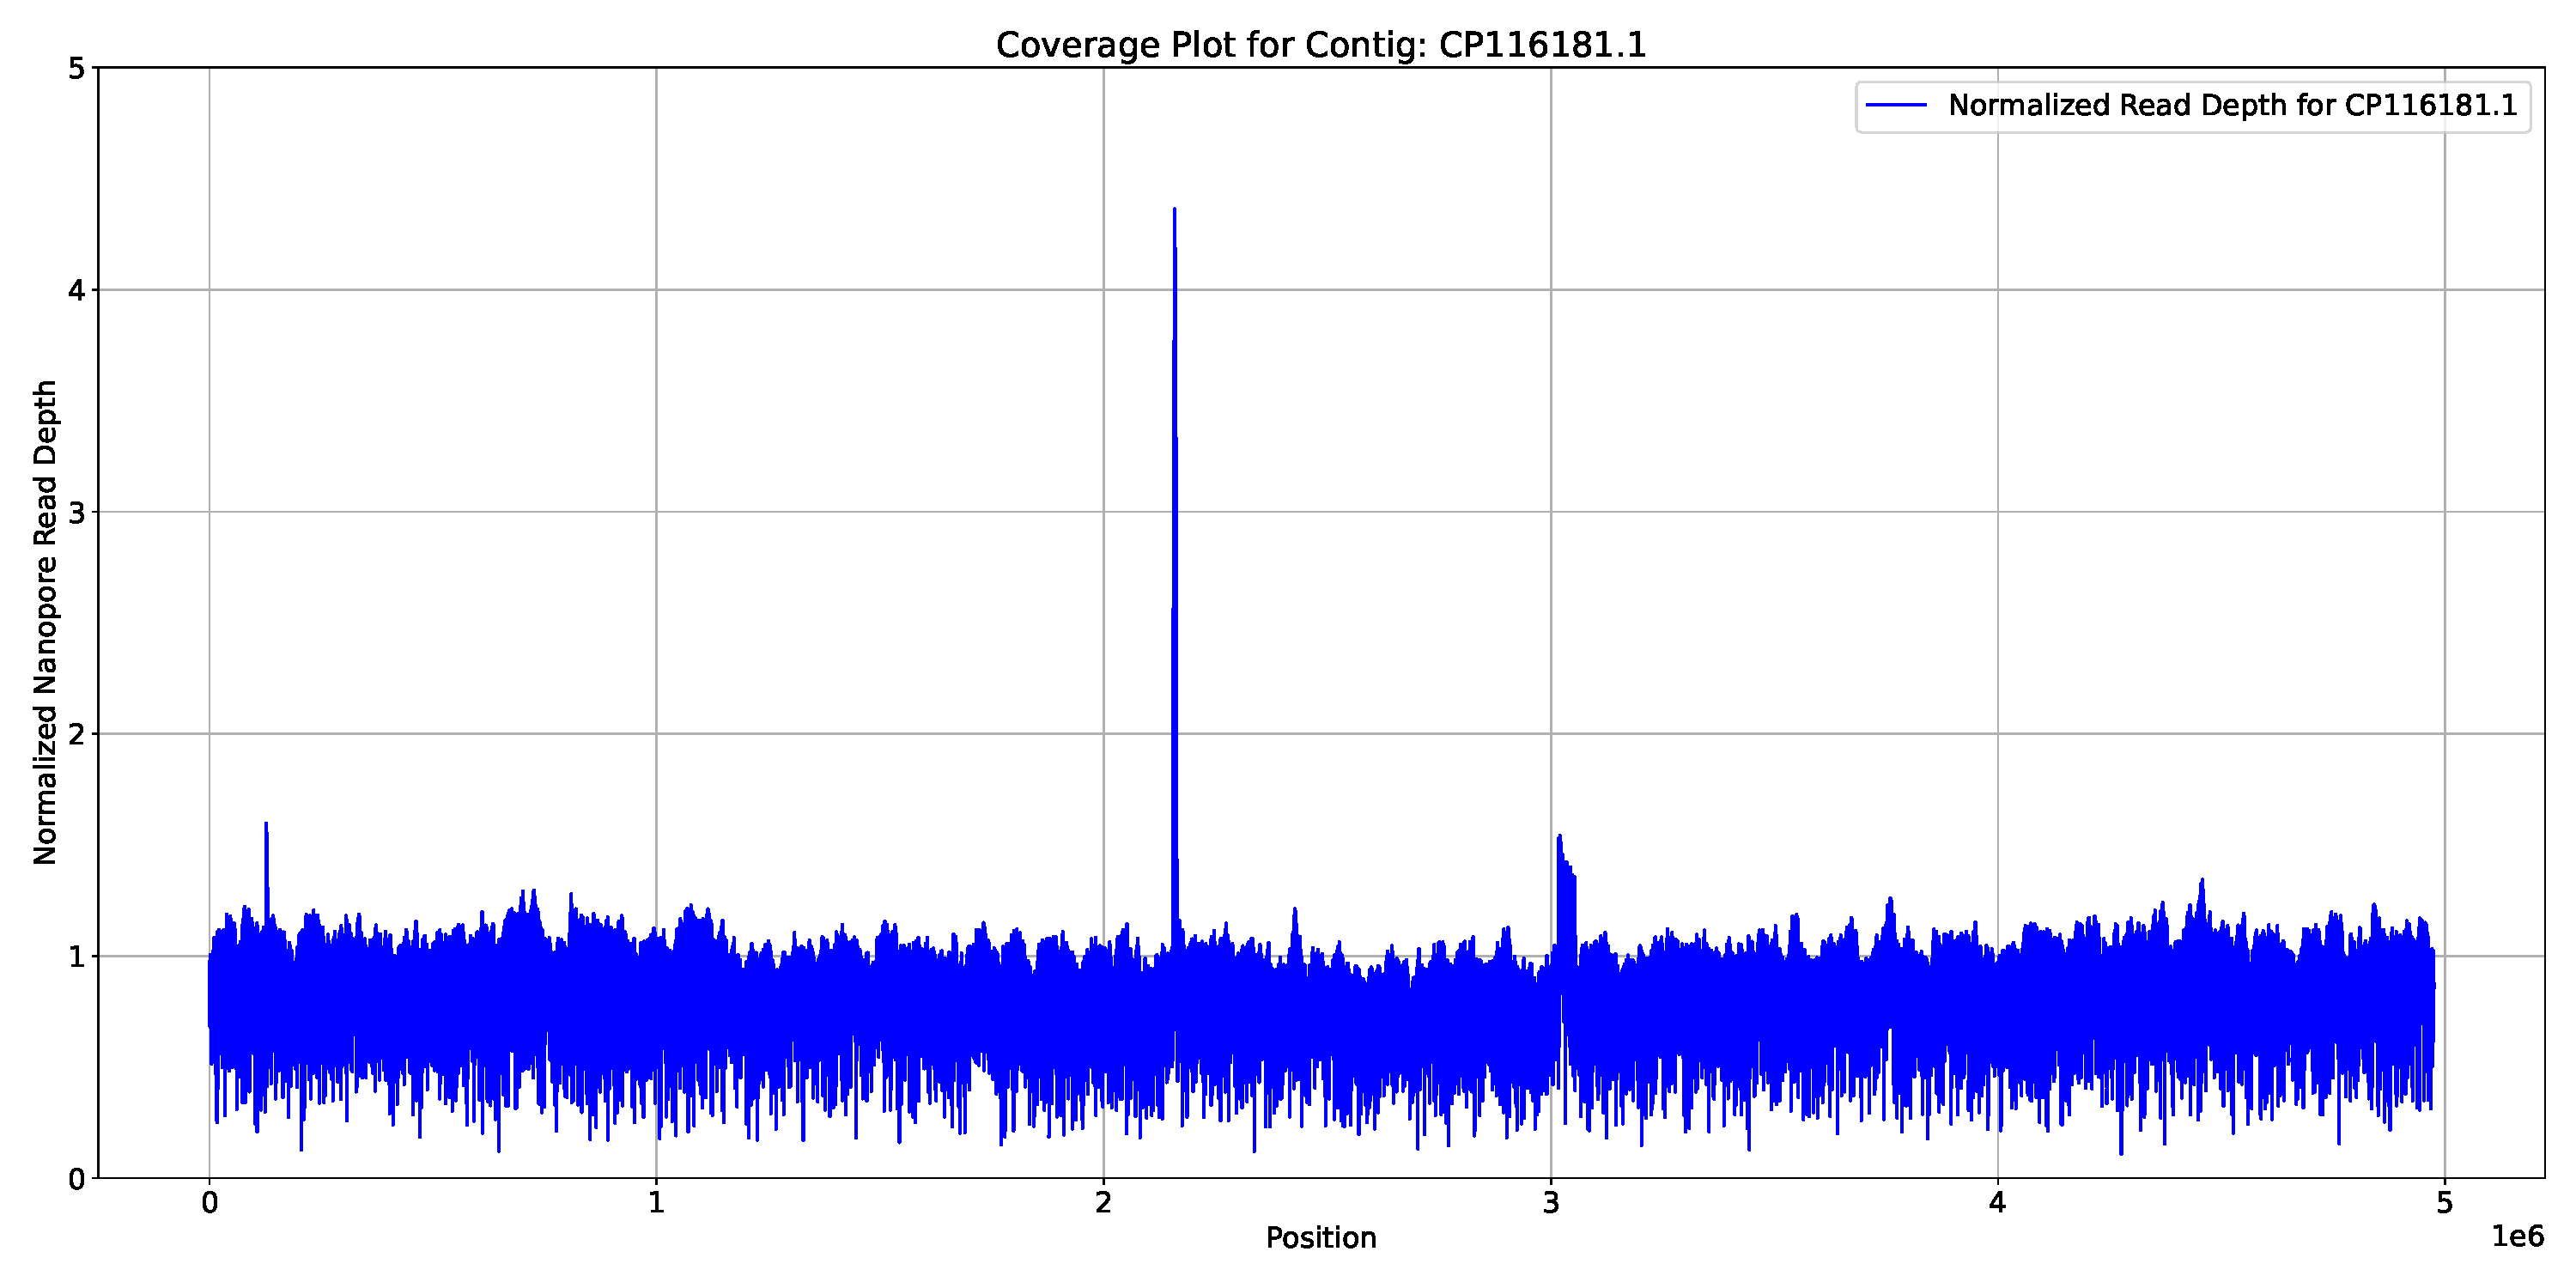
\includegraphics[width=0.75\linewidth]{Figures/figure_S5.pdf}
\caption{We identified a region of elevated coverage in contig CP116181.1 in sample GCA\_027944955.1\_ASM2794495v1\_genomic. We extracted the soft-clipped reads mapping to this region using \texttt{samtools view -f 2048 -f 2064 GCA\_027944955.1\_ASM2794495v1\_genomic.bam CP116181.1:2000000-2500000 | cut -f1 | sort | uniq} and subsetted the nanopore FASTQ to just these reads using pyfastaq \texttt{filter}. We reassembled the reads using flye \texttt{v2.9.3} \texttt{--iterations 3}. We visualised the alignment between the assembly and the reference using TNA \texttt{v0.3.0}, and found it fully covered plasmid contig CP116184.1 with identity 99.8\%, so was not evident of a collapsed duplication.}
\label{suppfig:5}
\end{figure*}

\begin{figure*}[!ht]
\centering
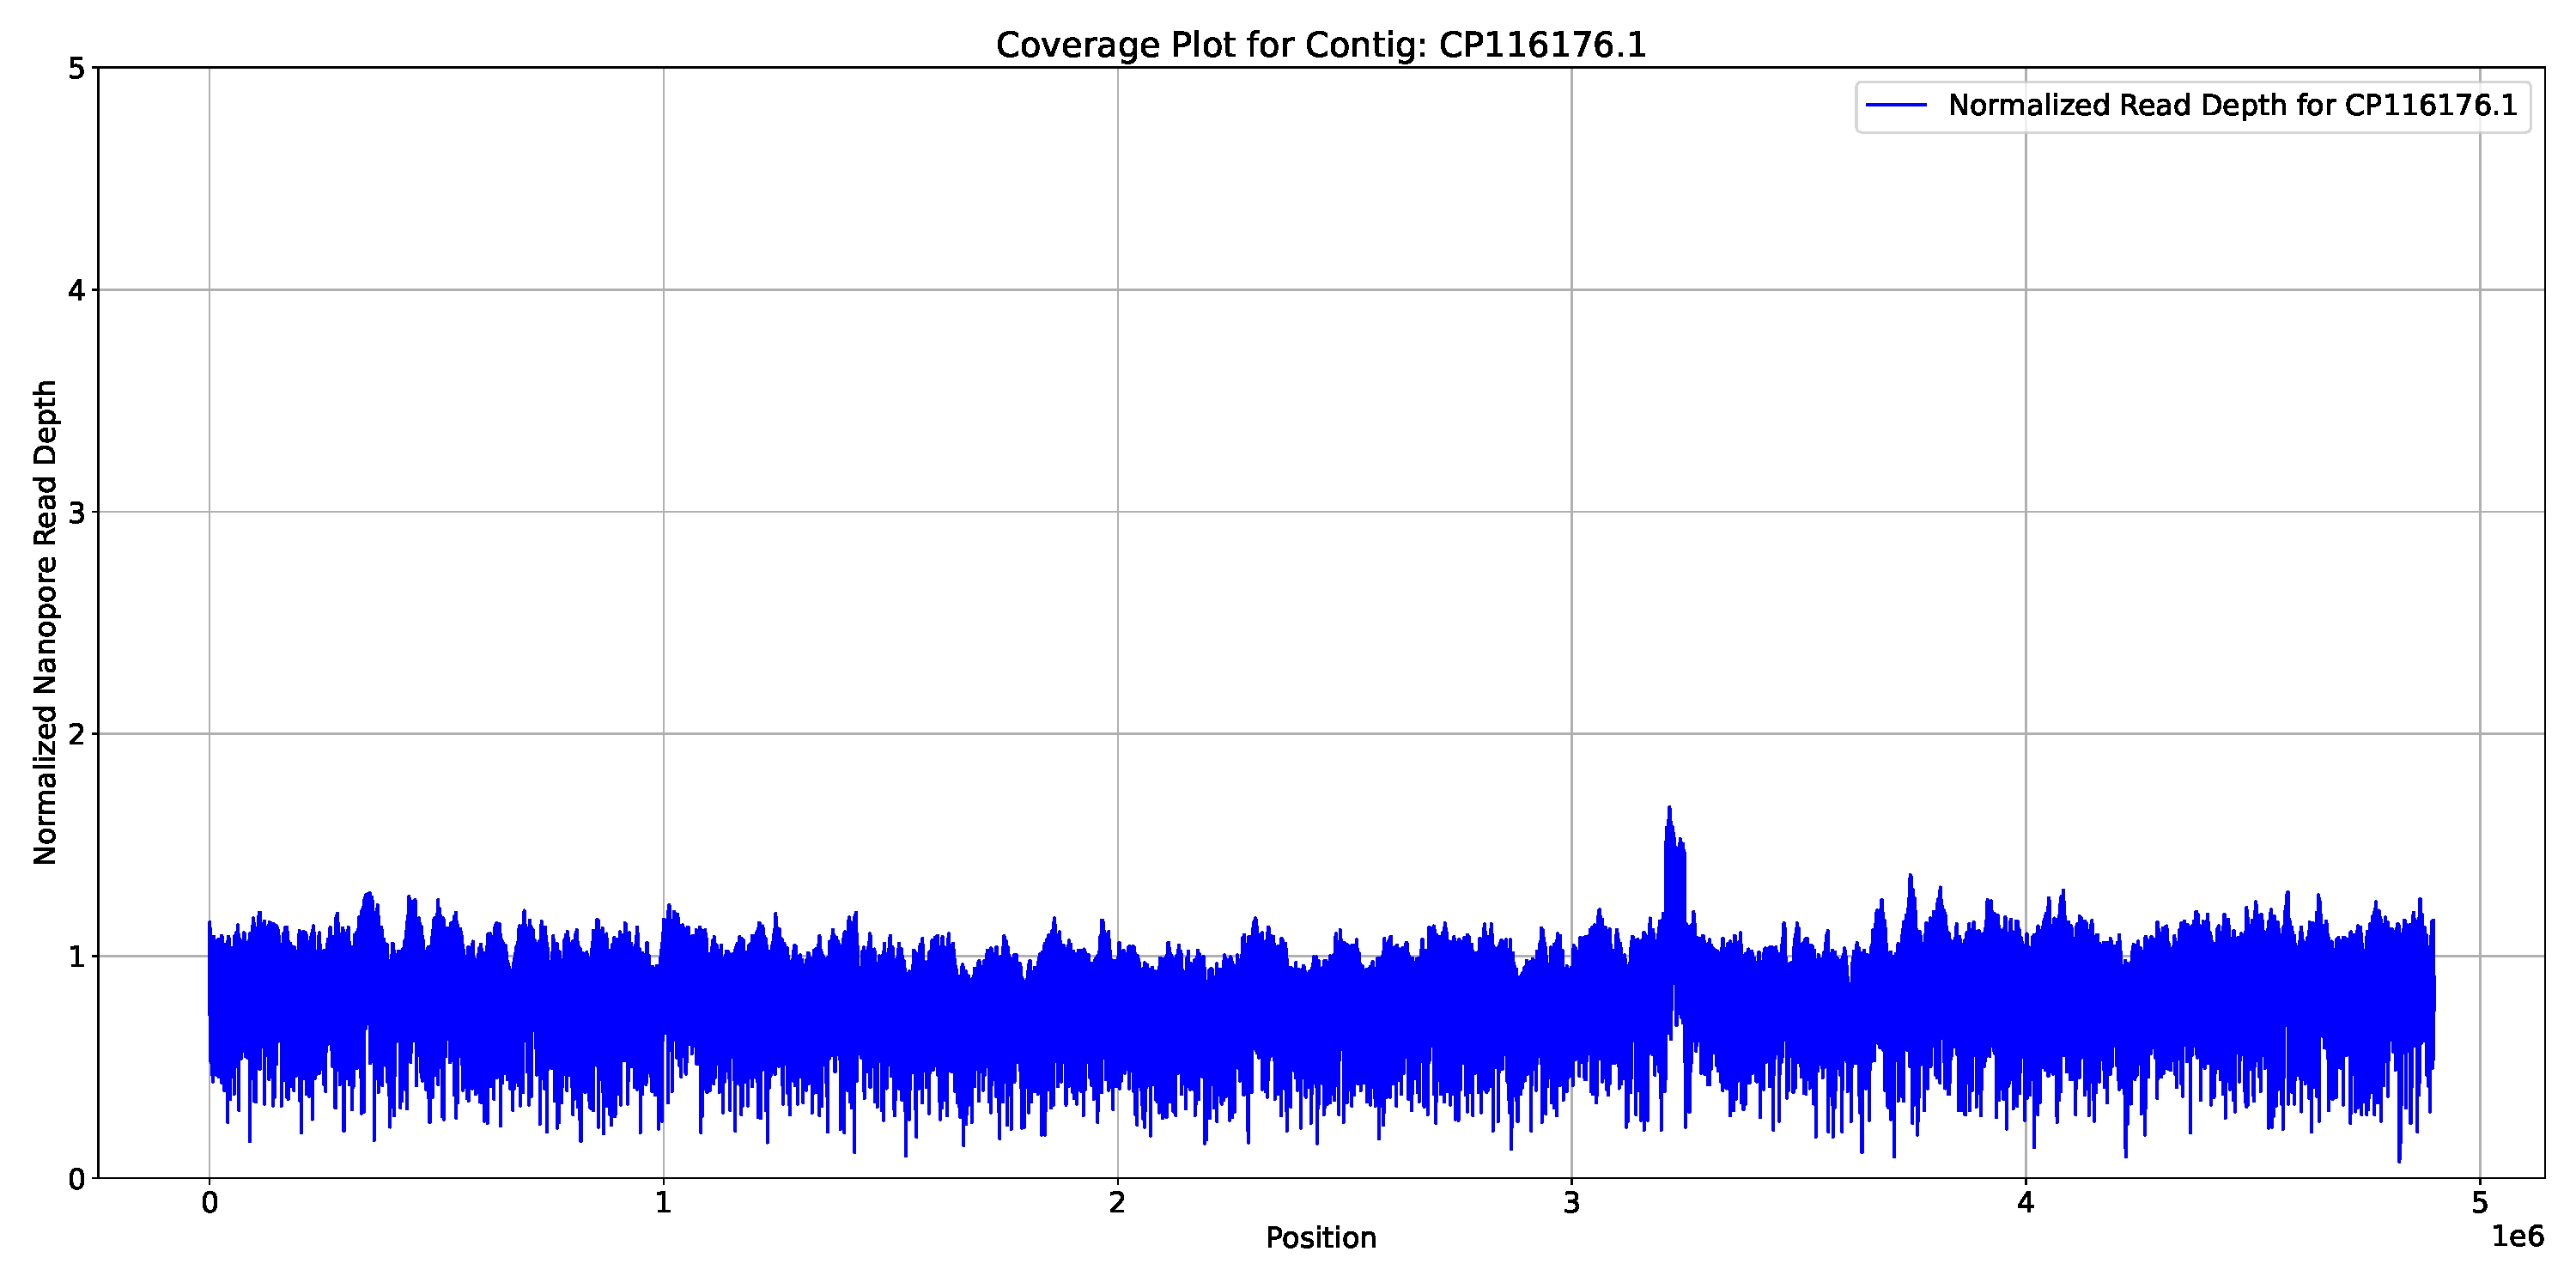
\includegraphics[width=0.75\linewidth]{Figures/figure_S2.pdf}
\caption{We identified a region of elevated coverage in contig CP116176.1 in sample GCA\_027944935.1\_ASM2794493v1\_genomic. We extracted the soft-clipped reads mapping to this region using \texttt{samtools view -f 2048 -f 2064 sample GCA\_027944935.1\_ASM2794493v1\_genomic.bam CP116176.1:3100000-35000000 | cut -f1 | sort | uniq} and subsetted the nanopore FASTQ to just these reads using pyfastaq \texttt{filter}. We reassembled the reads using flye \texttt{v2.9.3} \texttt{--iterations 3}. We visualised the alignment between the assembly and the reference using TNA \texttt{v0.3.0}, and found all generated contigs full aligned to the reference with >95\% identity.}
\label{suppfig:2}
\end{figure*}

\begin{figure*}[!ht]
\centering
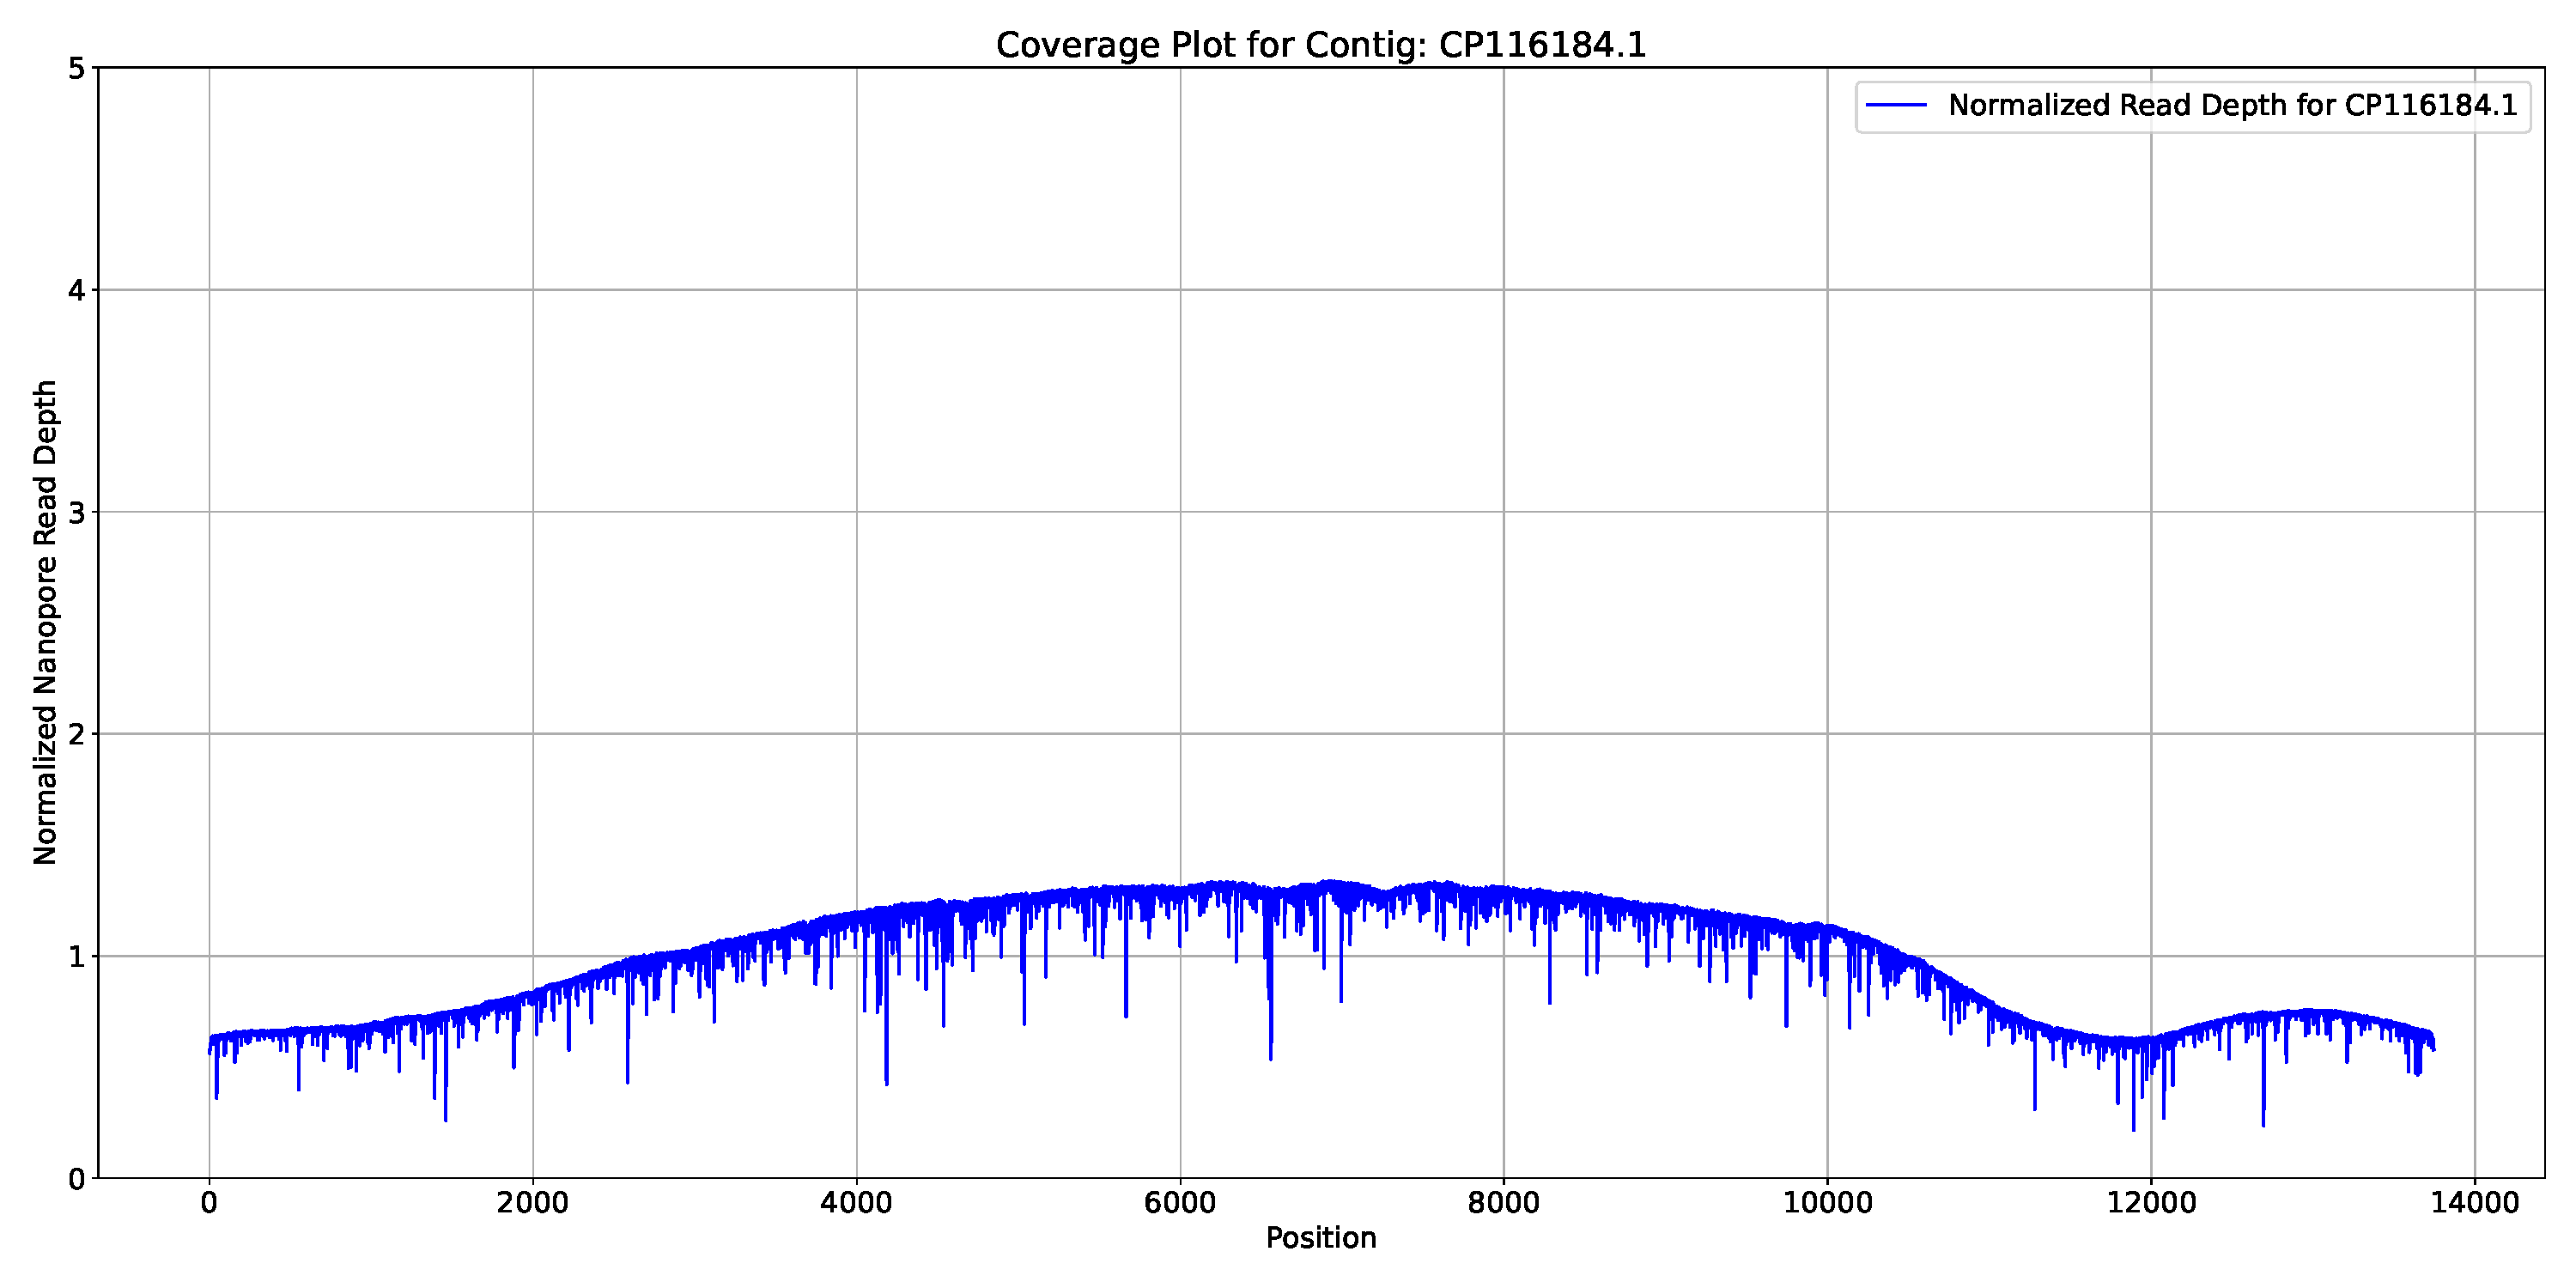
\includegraphics[width=0.75\linewidth]{Figures/figure_S6.pdf}
\caption{We identified a region of elevated coverage in contig CP116184.1 in sample GCA\_027944955.1\_ASM2794495v1\_genomic. We subsetted the reads mapping to the contig using \texttt{samtools view GCA\_027944955.1\_ASM2794495v1\_genomic.bam CP116184.1 | cut -f1 | sort | uniq} and pyfastaq \texttt{filter}. We reassembled the reads using Canu \texttt{v2.3} with \texttt{genomeSize=20k} and short-read polished the resulting contigs with polypolish \texttt{v0.6.0}. We then directly replaced CP116184.1 with the longest polished contig.}
\label{suppfig:6}
\end{figure*}

\begin{figure*}[!ht]
\centering
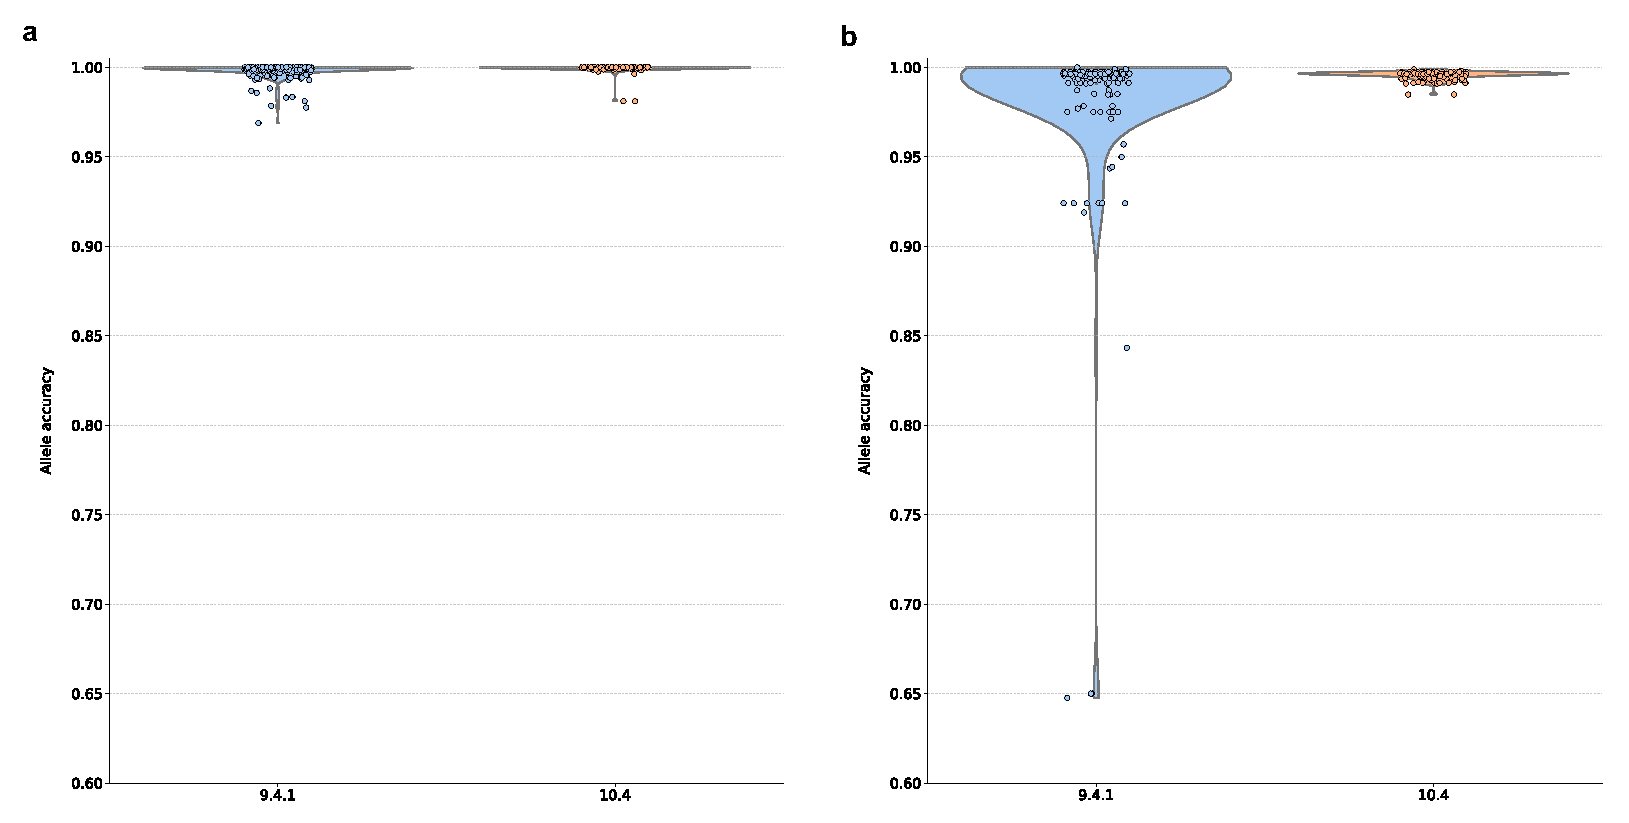
\includegraphics[width=1\linewidth]{Figures/figure_S7.pdf}
\caption{Violin plots comparing the gap-inclusive nucleotide similarities of alleles output by Amira (a) and assembled by Flye (b) on a truth dataset of 32 \textit{E. coli}.}
\label{suppfig:7}
\end{figure*}

\begin{figure*}[!ht]
\centering
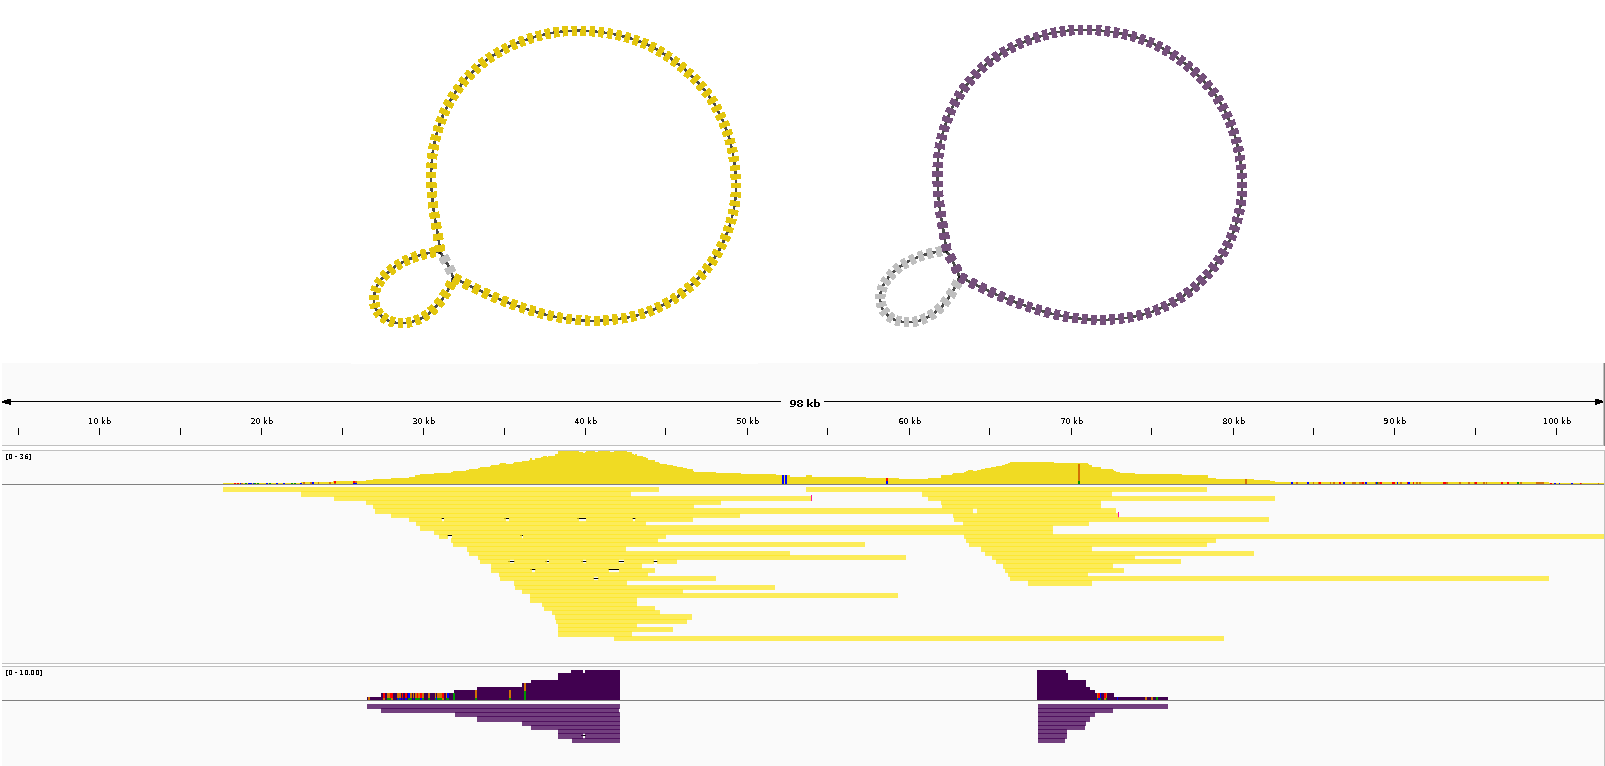
\includegraphics[width=1\linewidth]{Figures/figure_S8.pdf}
\caption{A comparison of two structural variants of the same plasmid in sample AUSMDU00021208, one version containing a 26.7\textit{kbp} mobile genetic element (yellow) and one version without it (purple). The variant without the element was missing from the reference assembly for this sample, resulting in Amira calling additional AMR gene copies due to an additional path through the connected component (top). We separated the reads unique to each path, mapped them to the reference and visualised the pileups with IGV to find two variants of the plasmid exist in the read set (bottom)}
\label{suppfig:8}
\end{figure*}